\documentclass[11pt]{article}
\usepackage[margin=0.8in]{geometry}
\usepackage[T1]{fontenc}
\usepackage{lmodern,graphicx,amsmath}
\usepackage[hidelinks]{hyperref}
\begin{document}
\title{Classical/Quantum Boundary Diagnostic}
\author{Research execution record}
\date{18 October 2026}
\maketitle
\noindent\textbf{Partial. No quantum execution or full Shor postprocessor.}

The native program emitted 75 resource rows and checked 18 exact-congruence
inputs: 15 recovered the chosen integer and three noninvertible zero
coefficients were rejected. Unit tests additionally cover every secret and
unit modulo 101 and a composite nonunit.

Resource rows keep public-point doublings, coordinate bytes, logical qubits
and Toffoli bounds separate. At 256 prime-field bits the RNSL 2017 formula
gives 2,330 logical qubits and approximately $1.287\times10^{11}$ Toffoli gates
per shot. Repeated-shot probabilities are explicitly assumed sensitivity
inputs. They are not measured circuit success probabilities.

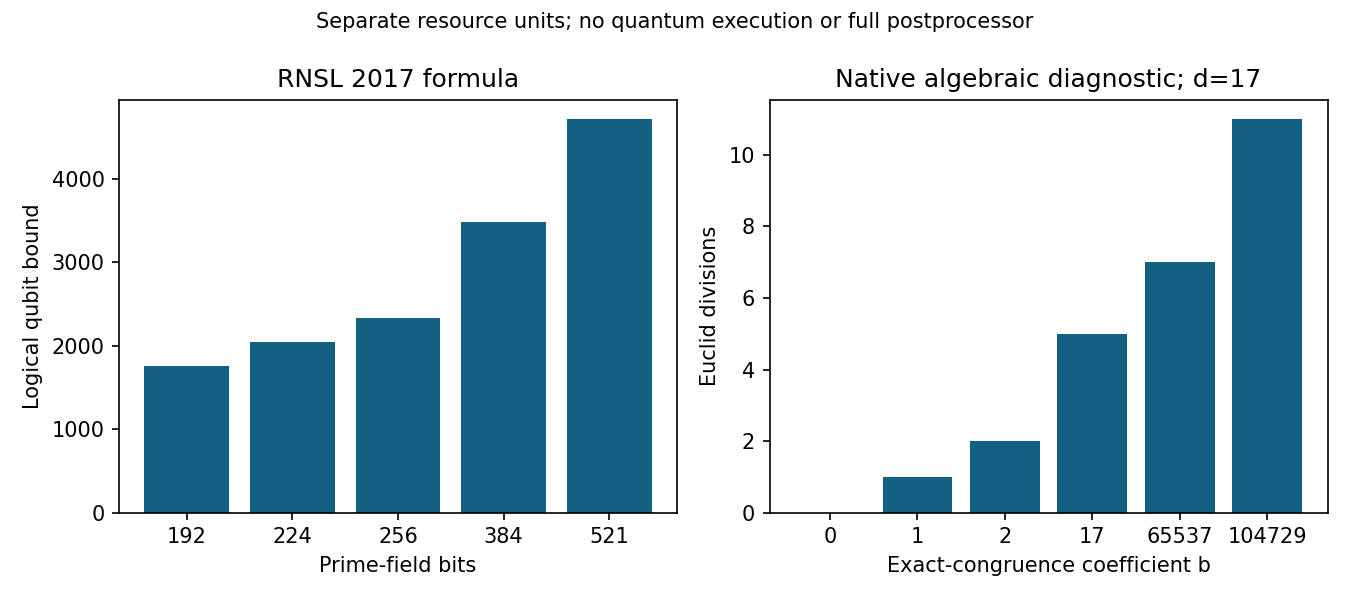
\includegraphics[width=\linewidth]{quantum_boundary.png}

The algebraic input $a+bd=0\pmod r$ is exact and synthetic. The experiment
does not recover this congruence from noisy power-of-two Fourier samples.
It does not time actual point tables, verify an elliptic-curve candidate,
simulate QFT/feed-forward, or estimate fault-tolerant physical resources.
These are remaining obligations for item 20.

\noindent\textbf{Evidence.} The frozen protocol, Rust source, 75 resource rows,
18 diagnostics, seven-test output and command/source manifest are retained
beside this report. Execution revision: \texttt{b3a3321c}.

\noindent\textbf{Sources.} Roetteler et al., arXiv:1706.06752 (2017);
H\"aner et al., arXiv:2001.09580 (2020), section 2. No gate counts from
different architectures are combined.
\newpage
\section*{Finite Fourier-output follow-up}
A separate frozen protocol calculates the actual power-of-two Fourier output
law on twelve synthetic cyclic groups: orders 5, 11 and 19, using transform
sizes 16, 32 and 64. The native code traces out the group register and Fourier
transforms every coset indicator. All laws normalize within $10^{-10}$.

The nearest-character decoder retains correct, incorrect and rejected
candidate masses. It is a heuristic with observed failures, not a complete
recovery algorithm. No small-group probability is transferred to deployed
parameters.

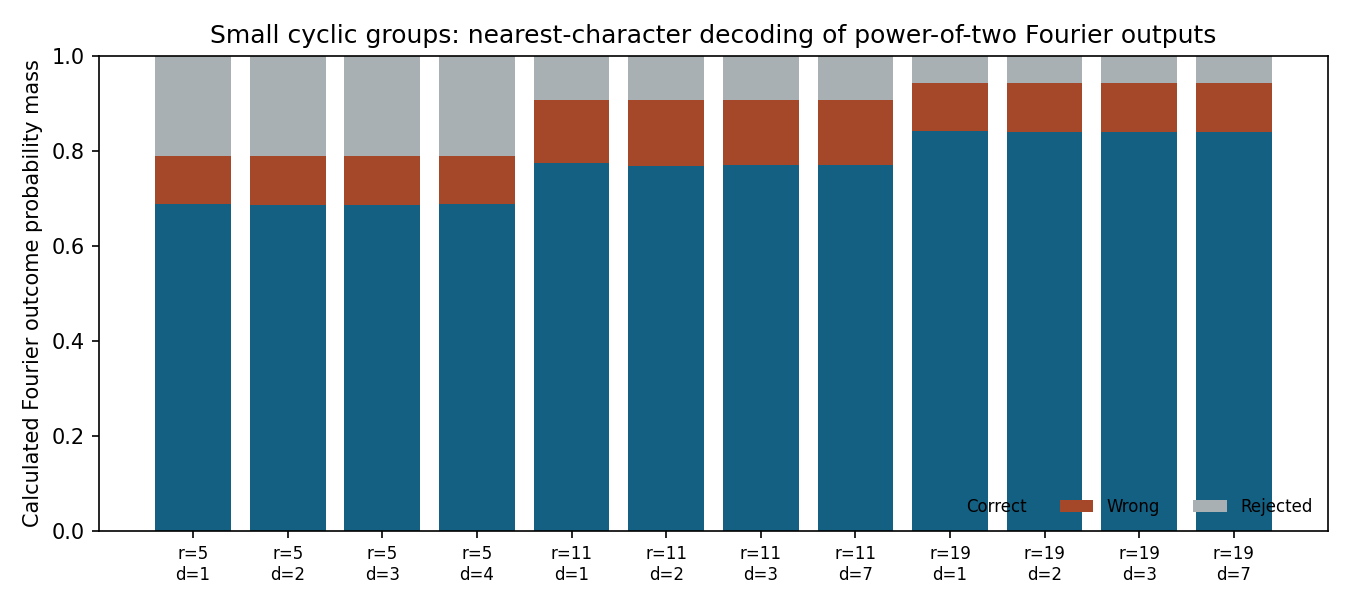
\includegraphics[width=\linewidth]{fourier_recovery.png}

Three additional tests pass, including comparison of the FFT with a naive
DFT and symmetry of the $d=1$ outcome law. The standalone crate now has ten
passing tests. This is classical numerical simulation of a small cyclic-group
distribution. Candidate checking uses the known synthetic integer and does
not execute elliptic-curve verification or a quantum circuit.

\noindent\textbf{Evidence.} Separate Fourier protocol, native source and all
twelve complete probability tables are retained in the campaign directory.
Source revision \texttt{b7528cb5}; binary \texttt{fourier-recovery}.
\end{document}
